
\chapter{Mise en \oe{}uvre de \PpFf}
\label{implementation.chap}


Ce chapitre décrit la fa\c{c}on dont \TT{PpFf} est impl\'ement\'e. 
%
De fa\c{c}on g\'en\'erale, la mise en \oe{}uvre utilise la biblioth\`eque \TT{FastFlow}, et ce en h\'eritant et \'etendant plusieurs de ses classes.

Ce chapitre est divis\'e en deux sections.
%
La premi\`ere section d\'ecrit les diff\'erents éléments composant la biblioth\`eque \TT{PpFf}, et la deuxi\`eme section pr\'esente quelques exemples d\'ecrivant comment un programme \PpFf{} est compil\'e et ex\'ecut\'e.


\section{Les \'el\'ements de \TT{PpFf}}

\begin{figure}
\centering
         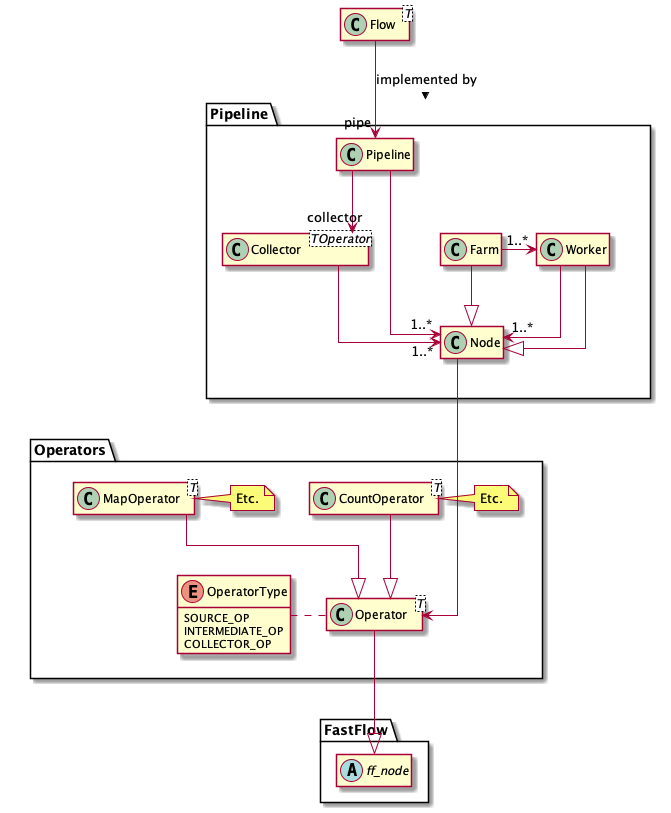
\includegraphics[width=1.0\textwidth]{Figures/vueEnsemble.png}
      \caption{Les principaux éléments (classes) de \TT{PpFf}.}
       \label{All.fig}
\end{figure}

La biblioth\`eque \TT{PpFf} est compos\'ee de plusieurs modules qui permettent de g\'erer les flux de traitement de donn\'ees. Une vue d'ensemble de ces modules est illustr\'ee dans la figure~\ref{All.fig}.

\begin{itemize}

\item Le point d'entr\'ee de \ppff\ est la classe \TT{Flow}, avec laquelle interagissent les d\'eveloppeurs pour cr\'eer des flux de traitement. Toutes les op\'erations de traitement d'un flux de \TT{PpFf} sont li\'ees aux m\'ethodes expos\'ees par cette classe. 

\item Le c\oe{}ur de la mise en \oe{}uvre de \TT{PpFf} est le module \TT{Pipeline}. La cr\'eation et l'ex\'ecution d'un flux sont g\'er\'ees par celui-ci, qui construit tout d'abord une représentation intermédaire, et qui génère ensuite un graphe de n\oe{}uds FastFlow.

\item  Le module \TT{Operators} regroupe tous les op\'erateurs d\'efinis dans \TT{PpFf}. Expos\'es \`a l'utilisateur par le biais de l'\TT{API} de \TT{PpFf}, ces op\'erateurs permettent de traiter les donn\'ees de diverses façons.

\item Le dernier module, \TT{FastFlow}, est la biblioth\`eque au–dessus de laquelle \TT{PpFf} est impl\'ement\'e.


\end{itemize}

\subsection{Flow}

\begin{figure}
\centering
     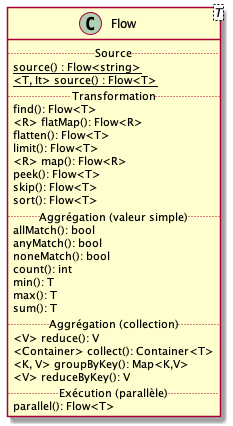
\includegraphics[width=0.5\textwidth]{Figures/flow-details.png}
      \caption{Les diff\'erentes m\'ethodes export\'ees par l'API de \TT{PpFf}.}
       \label{Flow.fig}
\end{figure}



La classe \TT{Flow} est celle qui définit l'\TT{API} de la biblioth\`eque \TT{PpFf}, l'interface avec laquelle interagit le d\'eveloppeur. La figure~\ref{Flow.fig} --- qui reprend la figure~\ref{MethodesAPI.fig} --- pr\'esente la vue d'ensemble des diverses m\'ethodes export\'ees par \TT{PpFf}. Selon le type export\'e par l'\TT{API}, les m\'ethodes sont divis\'ees en plusieurs groupes : Source, Transformation, Aggr\'egation (valeur simple ou collection) et Ex\'ecution (parallèle).

\begin{itemize}

\item Le premier groupe, Source, est le groupe de méthodes (statiques) qui permettent de créer un flux de donn\'ees. Ce sont es m\'ethodes qui fournissent les donn\'ees initiales pour un flux. Sans un appel \`a une telle m\'ethode, un flux ne peut pas exister. 

\item Le deuxi\`eme groupe, Transformation, est composé des m\'ethodes qui retournent une r\'ef\'erence vers un objet \TT{Flow}. C'est ce m\'ecanisme permet d'encha\^iner les m\'ethodes de l'\TT{API}.

\item Le troisi\`eme groupe, Aggr\'egation, est divis\'e en deux sous-groupes, selon le type de r\'esultat produit : valeur simple --- les m\'ethodes retournant une valeur simple, habituellement un scalaire (par ex., r\'esultat bool\'een ou entier) et collection --- les m\'ethodes retournant une collection.

\item Le quatrième et dernier groupe, Exécution, comporte une seule m\'ethode. Cette m\'ethode modifie le comportement d'ex\'ecution du flux. Lorsqu'elle est ajout\'ee au  \TT{pipeline}, toutes les op\'erations suivant cette m\'ethode seront ex\'ecut\'ees en parall\`ele, en utilisant les instances d'un  \TT{farm}.

L'\TT{API} de \TT{PpFf} permet d'appliquer plusieurs op\'erations les unes à la suite des autres sur une collection de donn\'ees. Ceci est possible en encha\^inant les m\'ethodes (\emph{method chaining}). Les m\'ethodes de l'\TT{API} peuvent \^etre enchain\'ees tant qu'elles retournent une r\'ef\'erence \`a \TT{Flow}. Lorsqu'une m\'ethode retourne une valeur, une valeur simple ou une collection, le traitement est alors ex\'ecut\'e. 

\end{itemize}





\begin{lstlisting}[
label={source.c++},
language=c++,
gobble=4,
caption={Extraits (squelette) de la classe \TT{Flow} avec la variable d'instance \TT{pipe} et le code de la m\'ethode statique \TT{soure}.},
frame=single,
float]
    class Flow {

    public:
        static Flow& source(const std::string& path) {
            typedef LinesFromFileOperator LinesFromFile;

            Flow* flow = new Flow();
            flow->pipe.addNodes<LinesFromFile>(1, path);

            return *flow;
        }

        // ... Autres methodes....
        // ... Voir autres listings pour des exemples...

    private:
        Pipeline pipe;
    };
\end{lstlisting}

\begin{lstlisting}[
label={count.c++},
language=c++,
gobble=7,
caption={Le code de la m\'ethode \TT{count} de la classe \TT{Flow}.},
frame=single,
float]
        unsigned int count() {
            typedef CountOperator<int> Count;
            
            pipe.addNodes<Count>(pipe.nbWorkers());
            pipe.run();

            return pipe.value<Count, int>();
        }
\end{lstlisting}

\GT{La méthode est tellement simple que tu es aussi bien de tout
donner son code! Tu peux faire un copier/coller du fichier Flow.hpp,
puis ajouter "gobble" si le code est trop indenté, pour le coller plus
à gauche.}

\IC{Je n'ai pas compris. Est-ce que je dois ajouter toutes les méthodes de Flow ?}

\GT{Non, je voulais simplement dire que tu pouvais fournir le code
complet pour la méthode \TT{count}: l'extrait que tu avais présenté
n'avait que 2-3 lignes de moins que la méthode complète. Donc, pour si peu de lignes, aussi bien présenté toute la méthode.}

\GT{Par contre, avec cette méthode, tu présentes une méthode du groupe
Aggrégation. Peut-être serait-il bien de  présenter aussi le code pour
une méthode du groupe Source (LinesFromFile?) et une méthode du groupe
Transformation (map?)?   En les présentant  dans le même ordre  que tu
présentes les groupes?!  J'ai ajouté le premier...}



L'\TT{API} de \TT{PpFf} est mise en œuvre par le module \TT{Pipeline}. Ce dernier s'occupe de la cr\'eation et de l'ex\'ecution du flux. Le listing~\ref{count.c++} pr\'esente le code de la m\'ethode \TT{count} de l'\TT{API}. L'attribut \TT{pipe} d'un objet \TT{Flow} est une instance de la classe \TT{Pipeline}, objet qui cr\'ee et ajoute les op\'erateurs de type \TT{Count} dans le pipeline associé au flux en appelant la m\'ethode \TT{addNodes}. Une fois les n\oe{}uds ajoutés, puisqu'il s'agit d'une méthode qui produit un résultat qui n'est pas un \TT{Flow}, le traitement associé au pipeline \TT{pipe} est ex\'ecut\'e en appelant la m\'ethode \TT{run}. Puis, on obtient et on retourne la valeur de type entier (\TT{int}, sp\'ecifi\'e dans le deuxi\`eme param\`etre générique de la m\'ethode \TT{value}) produit par l'exécution du pipeline.

\subsection{Pipeline}
\subsection{Opérateurs}


\section{Impl\'ementation de \TT{PpFf} avec \TT{FastFlow} : un exemple}


\begin{itemize}

\item objets1 

\item objets2 

\item objets3 


\end{itemize}
